% =============================================================================
%  ESI Journal Platform (OJS 3.5) -- Deployment and Operations Guide
%  Compile:  pdflatex ojs-deployment-guide.tex   (run twice for the table of contents)
%       or:  latexmk -pdf ojs-deployment-guide.tex
% =============================================================================
\documentclass[11pt,a4paper]{report}

% ---- Edit these before compiling --------------------------------------------
\newcommand{\DocTitle}{ESI Journal Platform}
\newcommand{\DocSubtitle}{Deployment and Operations Guide\\[2pt]\large Open Journal Systems 3.5 on Docker}
\newcommand{\DocVersion}{1.0}
\newcommand{\DocDate}{2 November 2026}
\newcommand{\DocAuthor}{Your Name}
\newcommand{\DocAudience}{ESI IT team}
% -----------------------------------------------------------------------------

\usepackage[T1]{fontenc}
\usepackage[utf8]{inputenc}
\usepackage{lmodern}
\usepackage[margin=2.3cm,headheight=14pt]{geometry}
\usepackage{microtype}
\usepackage[table]{xcolor}
\usepackage{graphicx}
\usepackage{array,booktabs,tabularx,longtable}
\usepackage{enumitem}
\usepackage{amssymb}
\usepackage{listings}
\usepackage[most]{tcolorbox}
\usepackage{tikz}
\usetikzlibrary{arrows.meta,positioning,fit,backgrounds}
\usepackage{fancyhdr}
\usepackage{titlesec}
\usepackage[hidelinks]{hyperref}

% ---- Colours ----------------------------------------------------------------
\definecolor{esiblue}{HTML}{0060B0}
\definecolor{codebg}{HTML}{F5F7FA}
\definecolor{coderule}{HTML}{C9D3DF}
\definecolor{notebg}{HTML}{EAF2FB}
\definecolor{warnbg}{HTML}{FDF1E7}
\definecolor{warnrule}{HTML}{D9822B}
\definecolor{rulebg}{HTML}{FBEAEA}
\definecolor{rulerule}{HTML}{B03A2E}
\definecolor{okgreen}{HTML}{2E7D32}

\hypersetup{colorlinks=true,linkcolor=esiblue,urlcolor=esiblue,
  pdftitle={\DocTitle{} -- Deployment and Operations Guide},pdfauthor={\DocAuthor}}

% ---- Headings, header/footer ------------------------------------------------
\titleformat{\chapter}[hang]{\normalfont\huge\bfseries\color{esiblue}}{\thechapter}{0.6em}{}
\titlespacing*{\chapter}{0pt}{-10pt}{18pt}
\titleformat{\section}{\normalfont\Large\bfseries\color{esiblue}}{\thesection}{0.6em}{}
\titleformat{\subsection}{\normalfont\large\bfseries}{\thesubsection}{0.6em}{}
\pagestyle{fancy}
\fancyhf{}
\fancyhead[L]{\small\color{gray}\DocTitle{} -- Deployment and Operations Guide}
\fancyhead[R]{\small\color{gray}v\DocVersion}
\fancyfoot[C]{\small\thepage}
\renewcommand{\headrulewidth}{0.3pt}
\fancypagestyle{plain}{\fancyhf{}\fancyfoot[C]{\small\thepage}\renewcommand{\headrulewidth}{0pt}}

\setlength{\parindent}{0pt}
\setlength{\parskip}{6pt}
\setlist{itemsep=2pt,topsep=4pt}
\renewcommand{\arraystretch}{1.25}
\newcolumntype{L}{>{\raggedright\arraybackslash}X}
\newcolumntype{P}[1]{>{\raggedright\arraybackslash}p{#1}}

% ---- Code -------------------------------------------------------------------
\lstdefinestyle{shell}{
  language=bash, basicstyle=\ttfamily\small, columns=fullflexible, keepspaces=true,
  upquote=true, breaklines=true, breakatwhitespace=false,
  postbreak=\mbox{\textcolor{gray}{$\hookrightarrow$}\space},
  backgroundcolor=\color{codebg}, frame=leftline, rulecolor=\color{coderule},
  framerule=2pt, xleftmargin=8pt, framexleftmargin=6pt, aboveskip=6pt, belowskip=6pt,
  showstringspaces=false, commentstyle=\color{gray}\itshape, keywordstyle={},
  stringstyle={}, morecomment=[l]{\#}}
\lstset{style=shell}
\lstnewenvironment{termout}{\lstset{style=shell,language={},commentstyle={},
  backgroundcolor=\color{white},frame=single,rulecolor=\color{coderule},framerule=0.4pt}}{}

% inline code: \code{...}  (escape _ $ % # & { } yourself)
\newcommand{\code}[1]{\texttt{\small #1}}
\newcommand{\file}[1]{\texttt{\small #1}}

% ---- Boxes ------------------------------------------------------------------
\newtcolorbox{note}[1][Note]{enhanced,breakable,colback=notebg,colframe=esiblue,
  boxrule=0pt,leftrule=3pt,arc=0pt,fonttitle=\bfseries,coltitle=esiblue,
  colbacktitle=notebg,title=#1,attach title to upper={\ --\ },before skip=8pt,after skip=8pt}
\newtcolorbox{warning}[1][Warning]{enhanced,breakable,colback=warnbg,colframe=warnrule,
  boxrule=0pt,leftrule=3pt,arc=0pt,fonttitle=\bfseries,coltitle=warnrule,
  colbacktitle=warnbg,title=#1,attach title to upper={\ --\ },before skip=8pt,after skip=8pt}
\newtcolorbox{rulebox}[1][Rules]{enhanced,breakable,colback=rulebg,colframe=rulerule,
  boxrule=0.6pt,arc=2pt,fonttitle=\bfseries,colbacktitle=rulerule,coltitle=white,title=#1,
  before skip=10pt,after skip=10pt}

\newcommand{\checkitem}{\item[$\square$]}

% =============================================================================
\begin{document}

% ---- Title page -------------------------------------------------------------
\begin{titlepage}
  \thispagestyle{empty}
  \vspace*{2cm}
  {\color{esiblue}\rule{\linewidth}{2pt}}\par\vspace{18pt}
  {\fontsize{30}{36}\selectfont\bfseries\color{esiblue}\DocTitle\par}
  \vspace{10pt}
  {\LARGE \DocSubtitle\par}
  \vspace{18pt}
  {\color{esiblue}\rule{\linewidth}{2pt}}\par
  \vspace{2.5cm}
  \begin{tabular}{@{}ll@{}}
    \textbf{Version}       & \DocVersion \\
    \textbf{Date}          & \DocDate \\
    \textbf{Prepared for}  & \DocAudience \\
    \textbf{Prepared by}   & \DocAuthor \\
    \textbf{Classification}& Internal -- contains no passwords \\
  \end{tabular}
  \vfill
  \begin{note}[About this document]
    This guide describes how the journal platform is built, from installing Docker on a fresh
    server to going live with a domain name, HTTPS and email, and how to run it day to day:
    backups, restores, monitoring, updates and troubleshooting.
    It contains no passwords. All secrets live in one file on the server (\file{.env}) and
    must be handed over in person.
  \end{note}
\end{titlepage}

% ---- Document control -------------------------------------------------------
\chapter*{Document control}
\addcontentsline{toc}{chapter}{Document control}
\begin{tabularx}{\linewidth}{@{}lllL@{}}
\toprule
\textbf{Version} & \textbf{Date} & \textbf{Author} & \textbf{Changes} \\
\midrule
1.0 & \DocDate & \DocAuthor & First release: installation, hardening, backups, domain/HTTPS, email, operations. \\
\bottomrule
\end{tabularx}

\vspace{12pt}
\textbf{Related files in the project repository}
\begin{itemize}
  \item \file{docs/OPERATIONS.md} -- short command reference (same content as Chapters~\ref{ch:ops} and~\ref{ch:trouble}).
  \item \file{docs/RESTORE.md} -- restore procedure (same content as Chapter~\ref{ch:backup}).
  \item \file{CHANGES.md} -- log of every manual change made to the deployment.
\end{itemize}

\tableofcontents

% =============================================================================
\chapter{Introduction}
% =============================================================================

\section{Purpose}
The ESI journal platform is a scientific journal website with an integrated submission and
peer-review workflow. It is built on \textbf{Open Journal Systems (OJS)}, the open-source
publishing software from the Public Knowledge Project (PKP), running in \textbf{Docker}
containers on a single Ubuntu virtual machine.

This guide is the reference for the team that installs, operates and maintains that server.
It covers:
\begin{itemize}
  \item installing the server and creating the containers (Chapters~\ref{ch:prereq}--\ref{ch:install});
  \item the security measures in place and the ones to finish before go-live (Chapter~\ref{ch:security});
  \item backups, restore tests and disaster recovery (Chapter~\ref{ch:backup});
  \item giving the journal its domain name with HTTPS, and enabling email (Chapters~\ref{ch:domain}--\ref{ch:email});
  \item daily operations, updates and troubleshooting (Chapters~\ref{ch:ops}--\ref{ch:trouble});
  \item a go-live checklist (Chapter~\ref{ch:golive}).
\end{itemize}

Editorial configuration of the journal (sections, review forms, editorial team, published
content) is done in the OJS web interface by the journal managers and is out of scope.

\section{Audience}
System and network administrators comfortable with the Linux command line, SSH and basic
Docker concepts (image, container, volume). No prior knowledge of OJS is required.

\section{Conventions}
\begin{itemize}
  \item Commands are run on the server as the administrator account (\code{spe} on the current
        VM), \textbf{from the project folder} \file{\textasciitilde/ojs-deploy}, unless stated otherwise.
        Commands that need root are written with \code{sudo}.
  \item Values in angle brackets are placeholders, e.g.\ \code{<domain>} or \code{<server-ip>}.
  \item Boxes: \textcolor{esiblue}{\textbf{Note}} = useful information;
        \textcolor{warnrule}{\textbf{Warning}} = risk of breaking something;
        \textcolor{rulerule}{\textbf{Rules}} = must always be followed.
\end{itemize}

\section{Current deployment at a glance}
\begin{tabularx}{\linewidth}{@{}P{4.6cm}L@{}}
\toprule
\textbf{Item} & \textbf{Value} \\
\midrule
Server (VM)            & hostname \code{SPE}, Ubuntu 22.04 LTS, 20 vCPU, 16~GB RAM, 491~GB disk \\
Addresses              & \code{10.0.3.31} (LAN), \code{10.184.150.225} (ZeroTier VPN); outbound traffic leaves through public IP \code{41.111.189.195} \\
Administrator account  & \code{spe} (SSH key login; member of the \code{sudo} and \code{docker} groups) \\
Project folder         & \file{/home/spe/ojs-deploy} (a clone of the project Git repository) \\
Journal URL (current)  & \code{http://10.0.3.31:8080/esi/} -- journal path \code{esi} \\
Software               & OJS 3.5.0-5 (image \code{pkpofficial/ojs:\allowbreak stable-3\_5\_0}, PHP 8.3, Apache 2.4); MariaDB 11.8 \\
Docker                 & Docker Engine 29.9, Docker Compose v5.6 \\
Compose project        & \code{ojs} -- containers \code{pkp\_app\_ojs}, \code{pkp\_db\_ojs} (and \code{pkp\_proxy\_ojs} once a domain is configured) \\
Backups                & \file{/home/spe/ojs-backups} on the VM; off-site copies pulled to the administrator's PC \\
Time zone              & Africa/Algiers (server, PHP and OJS); clock synchronised with NTP server \code{10.0.3.254} \\
\bottomrule
\end{tabularx}

% =============================================================================
\chapter{Architecture}\label{ch:arch}
% =============================================================================

\section{Components}
\begin{tabularx}{\linewidth}{@{}P{3.2cm}P{4.2cm}L@{}}
\toprule
\textbf{Container} & \textbf{Image} & \textbf{Role} \\
\midrule
\code{pkp\_app\_ojs}   & \code{pkpofficial/ojs:\allowbreak stable-3\_5\_0} & Apache 2.4 + PHP 8.3 + OJS. Serves the website on container port 80, published on the host as port \textbf{8080}. \\
\code{pkp\_db\_ojs}    & \code{mariadb:11.8} & Database. Reachable only from the internal Docker network (no published port). \\
\code{pkp\_proxy\_ojs} & \code{caddy:2.10} & \textit{Optional, added by \file{scripts/setup-domain.sh}.} Reverse proxy on ports 80/443 for the domain name; obtains and renews the HTTPS certificate automatically. \\
\bottomrule
\end{tabularx}

All containers use the restart policy \code{unless-stopped}: they start automatically when
Docker starts (for example after a reboot) unless an administrator stopped them on purpose.
Each container has a health check, visible with \code{docker compose ps}.

\section{Overview diagram}
\begin{center}
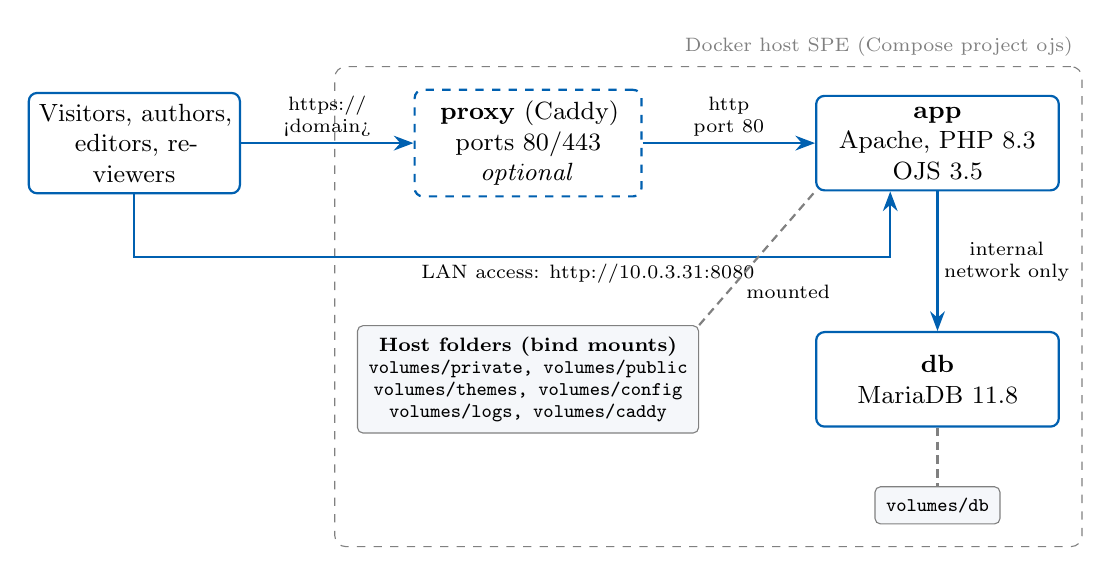
\begin{tikzpicture}[
    font=\small,
    box/.style={draw=esiblue,thick,rounded corners=3pt,fill=white,align=center,
                minimum height=1.2cm,text width=#1,inner sep=4pt},
    box/.default=2.6cm,
    vol/.style={draw=gray,rounded corners=2pt,fill=codebg,align=center,
                font=\scriptsize\ttfamily,inner sep=4pt},
    arr/.style={-{Stealth[length=2.5mm]},thick,draw=esiblue},
    dep/.style={densely dashed,thick,draw=gray},
    lab/.style={font=\scriptsize,align=center,inner sep=2pt}]
  % row 1: traffic
  \node[box=2.4cm] (users) at (0,0)    {Visitors, authors,\\editors, reviewers};
  \node[box=2.6cm,dashed] (proxy) at (5,0) {\textbf{proxy} (Caddy)\\ports 80/443\\\textit{optional}};
  \node[box=2.8cm] (app)   at (10.2,0) {\textbf{app}\\Apache, PHP 8.3\\OJS 3.5};
  % row 2: data
  \node[vol] (vols) at (5,-3) {{\normalfont\bfseries Host folders (bind mounts)}\\
        volumes/private, volumes/public\\volumes/themes, volumes/config\\volumes/logs, volumes/caddy};
  \node[box=2.8cm] (db)    at (10.2,-3) {\textbf{db}\\MariaDB 11.8};
  \node[vol] (vdb) at (10.2,-4.6) {volumes/db};
  % arrows
  \draw[arr] (users) -- node[lab,above]{https://\\<domain>} (proxy);
  \draw[arr] (proxy) -- node[lab,above]{http\\port 80} (app);
  \draw[arr] (users.south) -- ++(0,-0.8) -| node[lab,below,pos=0.3]{LAN access: http://10.0.3.31:8080}
        ([xshift=-6mm]app.south);
  \draw[arr] (app) -- node[lab,right]{internal\\network only} (db);
  \draw[dep] (vols.north east) -- node[lab,below right,pos=0.35]{mounted} (app.south west);
  \draw[dep] (db) -- (vdb);
  \begin{scope}[on background layer]
    \node[draw=gray,dashed,rounded corners=4pt,fit=(proxy)(app)(vols)(db)(vdb),inner sep=8pt,
          label={[font=\scriptsize\color{gray},anchor=south east]north east:Docker host SPE (Compose project ojs)}] {};
  \end{scope}
\end{tikzpicture}
\end{center}

\section{Network ports}
\begin{tabularx}{\linewidth}{@{}lllL@{}}
\toprule
\textbf{Port} & \textbf{Where} & \textbf{Who uses it} & \textbf{Notes} \\
\midrule
22/tcp   & host               & administrators     & SSH, key authentication. \\
8080/tcp & host $\to$ app:80  & LAN users          & Direct access by IP. Can be restricted to the server itself once the domain works (Chapter~\ref{ch:domain}). \\
80/tcp   & host $\to$ proxy   & internet           & Only after \file{setup-domain.sh}. HTTP, redirects to HTTPS; needed for certificate issuance. \\
443/tcp+udp & host $\to$ proxy & internet          & Only after \file{setup-domain.sh} with HTTPS. \\
9993/udp & host               & ZeroTier           & VPN used to reach the VM remotely. \\
3306/tcp & db (internal)      & app container only & \textbf{Not} published on the host. \\
\bottomrule
\end{tabularx}

\begin{note}
Ports published by Docker (8080, 80, 443) are opened by Docker's own firewall rules and are
\emph{not} filtered by \code{ufw}. To restrict them, bind them to \code{127.0.0.1} (the domain
script offers this for 8080) or filter them upstream.
\end{note}

\section{Data and persistence}\label{sec:volumes}
All data lives in folders of the project directory, mounted into the containers
(\emph{bind mounts}). Removing or recreating a container never deletes them.

\begin{tabularx}{\linewidth}{@{}P{5.3cm}P{5.7cm}L@{}}
\toprule
\textbf{Host path (in \file{\textasciitilde/ojs-deploy})} & \textbf{Container path} & \textbf{Content} \\
\midrule
\file{volumes/db/}            & db: \file{/var/lib/mysql}          & Database files. Backed up as a SQL dump, never copied raw. \\
\file{volumes/private/}       & app: \file{/var/www/files}         & Submissions, review files, galleys (PDF), usage statistics. \\
\file{volumes/public/}        & app: \file{/var/www/html/public}   & Public uploads: logos, cover images. \\
\file{volumes/themes/custom-theme/} & app: \file{.../plugins/themes/customTheme} & The ESI custom theme (tracked in Git). \\
\file{volumes/config/}        & app: single files                  & \file{config.inc.php}, \file{php.custom.ini}, \file{.htaccess}, Apache security config, DB charset config, \file{Caddyfile}. \\
\file{volumes/logs/}          & app: \file{/var/log/apache2}       & Apache log files, \file{health.log}, reports of the setup scripts. \\
\file{volumes/caddy/}         & proxy: \file{/data}, \file{/config} & HTTPS certificates and the Let's Encrypt account (once HTTPS is enabled). \\
\bottomrule
\end{tabularx}

\section{Configuration model}\label{sec:configmodel}
OJS reads its settings from \file{config.inc.php}. On this platform that file is
\textbf{generated} and must not be edited by hand:

\begin{center}
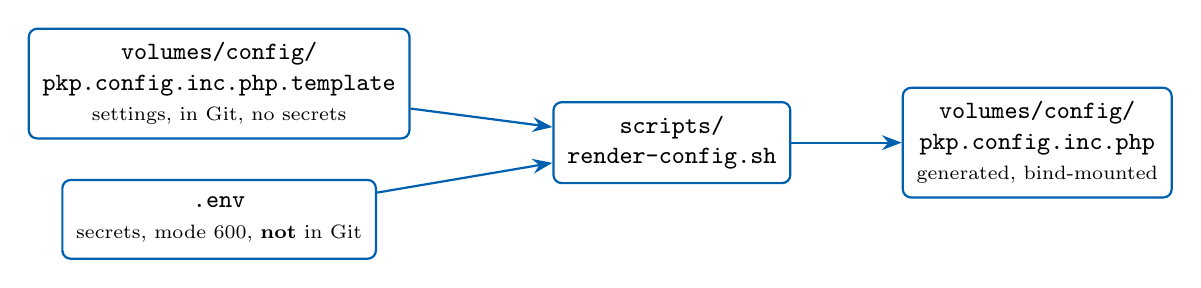
\begin{tikzpicture}[font=\small,
  b/.style={draw=esiblue,thick,rounded corners=3pt,align=center,inner sep=5pt,minimum height=1cm},
  arr/.style={-{Stealth[length=2.5mm]},thick,draw=esiblue}]
  \node[b] (t) {\file{volumes/config/}\\\file{pkp.config.inc.php.template}\\\scriptsize settings, in Git, no secrets};
  \node[b,below=0.5cm of t] (e) {\file{.env}\\\scriptsize secrets, mode 600, \textbf{not} in Git};
  \node[b,right=1.8cm of t,yshift=-0.75cm] (r) {\file{scripts/}\\\file{render-config.sh}};
  \node[b,right=1.4cm of r] (c) {\file{volumes/config/}\\\file{pkp.config.inc.php}\\\scriptsize generated, bind-mounted};
  \draw[arr] (t) -- (r); \draw[arr] (e) -- (r); \draw[arr] (r) -- (c);
\end{tikzpicture}
\end{center}

The template contains placeholders such as \code{\$\{OJS\_SALT\}}. The render script fills them
in from \file{.env} and writes the result into the running container \emph{in place}. Two reasons
for this design:
\begin{enumerate}
  \item OJS's configuration parser does not expand environment variables, so secrets cannot
        simply be referenced; they must be written into the file.
  \item The template can be versioned in Git without exposing any secret.
\end{enumerate}

\textbf{Secrets and where they live} (all in \file{.env} only):
\begin{tabularx}{\linewidth}{@{}P{4.6cm}L@{}}
\toprule
\textbf{\file{.env} key} & \textbf{Purpose} \\
\midrule
\code{MYSQL\_ROOT\_PASSWORD} & MariaDB root password. \\
\code{MYSQL\_PASSWORD}       & Password of the OJS database user (\code{pkp}); also copied to \code{DB\_PASS} and \code{PKP\_DB\_PASSWORD}. \\
\code{OJS\_APP\_KEY}          & OJS application encryption key, generated by the installer. \textbf{Never change it}: encrypted data would become unreadable. \\
\code{OJS\_SALT}              & OJS security salt (password-reset links, access keys). \\
\code{OJS\_API\_KEY\_SECRET}  & Secret used to sign OJS API tokens. \\
\code{OJS\_SMTP\_USER}, \code{OJS\_SMTP\_PASSWORD} & Gmail account and App Password (after Chapter~\ref{ch:email}). \\
\bottomrule
\end{tabularx}

\section{Repository layout}
\begin{tabularx}{\linewidth}{@{}P{5.6cm}L@{}}
\toprule
\textbf{Path} & \textbf{Content} \\
\midrule
\file{docker-compose.yml}          & Definition of the \code{app} and \code{db} services. \\
\file{docker-compose.proxy.yml}    & The optional Caddy proxy (enabled by \file{setup-domain.sh}). \\
\file{.env.example}                & Template for \file{.env} (placeholders only). \\
\file{volumes/config/}             & Configuration template and the small config files mounted into the containers. \\
\file{volumes/themes/custom-theme/}& The ESI theme. \\
\file{scripts/}                    & Operations scripts (Appendix~\ref{app:scripts}). \\
\file{docs/}                       & This guide, \file{OPERATIONS.md}, \file{RESTORE.md}. \\
\file{CHANGES.md}                  & Log of manual changes. \\
\bottomrule
\end{tabularx}

\section{Golden rules}\label{sec:rules}
\begin{rulebox}[Golden rules -- always follow them]
\begin{enumerate}[leftmargin=*]
  \item Run \code{docker compose} commands \textbf{from \file{\textasciitilde/ojs-deploy}}. The
        \file{.env} file there sets the project name \code{ojs}; from another folder, Compose
        does not see the containers.
  \item Apply configuration changes with \code{docker compose restart app}. \textbf{Never} use
        \code{docker compose down -v} (deletes volumes) and never delete anything under
        \file{volumes/}. Prefer \code{restart} to \code{up --force-recreate}.
  \item \textbf{Never edit \file{volumes/config/\allowbreak pkp.config.inc.php}}: edit the template and run
        \file{scripts/render-config.sh} (Section~\ref{sec:configchange}).
  \item Single files mounted into containers must be edited \emph{in place} (text editor or
        \code{cat > file}). \textbf{Never use \code{sed -i} or \code{mv}} on them: the container
        would keep seeing the old file.
  \item \textbf{Never run the image's \code{pkp-variable} helper}: it rewrites the config with
        \code{sed -i} and sets \code{installed = Off}, which breaks the site.
  \item Take a backup (\file{scripts/backup.sh}) before any change.
  \item Never copy secrets into e-mails, chat, tickets, scripts or Git. They belong in \file{.env} only.
\end{enumerate}
\end{rulebox}

% =============================================================================
\chapter{Prerequisites}\label{ch:prereq}
% =============================================================================

\section{Server}
\begin{tabularx}{\linewidth}{@{}lLL@{}}
\toprule
 & \textbf{Minimum} & \textbf{Current VM} \\
\midrule
CPU    & 2 vCPU   & 20 vCPU \\
Memory & 4 GB     & 16 GB \\
Disk   & 40 GB (plus room for uploads and backups) & 491 GB \\
OS     & Ubuntu 22.04 or 24.04 LTS, 64-bit & Ubuntu 22.04.5 LTS \\
\bottomrule
\end{tabularx}

An administrator account with \code{sudo} rights is needed. Do not run the platform as \code{root}.

\section{Network requirements}\label{sec:netreq}
\begin{tabularx}{\linewidth}{@{}lP{4.2cm}L@{}}
\toprule
\textbf{Direction} & \textbf{Destination / port} & \textbf{Why} \\
\midrule
Inbound  & 22/tcp from admin networks & SSH administration. \\
Inbound  & 8080/tcp from the LAN      & Access by IP address. \\
Inbound  & 80/tcp and 443/tcp from the internet & Domain name + HTTPS (Chapter~\ref{ch:domain}); port 80 is required for Let's Encrypt validation. \\
Outbound & Docker Hub (\code{registry-1.docker.io}, HTTPS) & Downloading the container images. \\
Outbound & \code{github.com} (HTTPS)     & Cloning / updating the project repository. \\
Outbound & Ubuntu mirrors (HTTP/HTTPS)  & OS security updates. \\
Outbound & \code{smtp.gmail.com} 587/tcp & Sending email (Chapter~\ref{ch:email}). \\
Outbound & Let's Encrypt (\code{acme-v02.api.\allowbreak letsencrypt.org}, HTTPS) & Obtaining/renewing certificates. \\
Outbound & HTTPS to the internet       & OJS scheduled tasks download reference data (ROR registry, IP geolocation database). \\
Outbound & NTP, UDP 123 to \code{10.0.3.254} & Clock synchronisation (public NTP servers are blocked on this network). \\
\bottomrule
\end{tabularx}

\section{External services}
\begin{itemize}
  \item \textbf{Domain name} (Chapter~\ref{ch:domain}): a DNS \code{A} record pointing to a public IP
        address whose ports 80 and 443 are forwarded to the VM.
  \item \textbf{Google account for email} (Chapter~\ref{ch:email}): an account with 2-Step Verification
        and an App Password. For a Google Workspace account, the Workspace administrator must
        allow App Passwords.
\end{itemize}

% =============================================================================
\chapter{Preparing the server}\label{ch:host}
% =============================================================================

\section{Update the operating system}
\begin{lstlisting}
sudo apt update && sudo apt full-upgrade -y
sudo reboot            # if a new kernel was installed
\end{lstlisting}

\section{Install Docker Engine and Docker Compose}
Use Docker's official repository (the \code{docker.io} package from Ubuntu is older):
\begin{lstlisting}
sudo apt install -y ca-certificates curl git python3 gettext-base
sudo install -m 0755 -d /etc/apt/keyrings
sudo curl -fsSL https://download.docker.com/linux/ubuntu/gpg -o /etc/apt/keyrings/docker.asc
sudo chmod a+r /etc/apt/keyrings/docker.asc
echo "deb [arch=$(dpkg --print-architecture) signed-by=/etc/apt/keyrings/docker.asc] \
https://download.docker.com/linux/ubuntu $(. /etc/os-release && echo "$VERSION_CODENAME") stable" \
  | sudo tee /etc/apt/sources.list.d/docker.list > /dev/null
sudo apt update
sudo apt install -y docker-ce docker-ce-cli containerd.io docker-buildx-plugin docker-compose-plugin
sudo systemctl enable --now docker
docker --version && docker compose version
\end{lstlisting}
\code{gettext-base} provides \code{envsubst} and \code{python3} is used by the scripts.

\section{Allow the administrator account to use Docker}
\begin{lstlisting}
sudo usermod -aG docker spe        # replace spe with the admin account
# log out and back in, then check:
docker ps
\end{lstlisting}
\begin{warning}
Members of the \code{docker} group can obtain root privileges on the host. Only trusted
administrators should be in this group.
\end{warning}

\section{SSH key access for administrators}
On the administrator's computer, create a key once and install it on the server:
\begin{lstlisting}
# Linux / macOS
ssh-keygen -t ed25519
ssh-copy-id spe@10.0.3.31

# Windows PowerShell
ssh-keygen -t ed25519
type $env:USERPROFILE\.ssh\id_ed25519.pub | ssh spe@10.0.3.31 "umask 077; mkdir -p ~/.ssh; cat >> ~/.ssh/authorized_keys"
\end{lstlisting}
Check that \code{ssh spe@10.0.3.31} no longer asks for a password. Password logins are disabled
later (Section~\ref{sec:sshhardening}); key access must work first.

% =============================================================================
\chapter{Creating the containers}\label{ch:containers}
% =============================================================================

\begin{note}[Two paths]
This chapter and the next one install a \textbf{new, empty} journal. To rebuild the
\textbf{existing} journal on a new server (migration or disaster recovery), follow
Section~\ref{sec:newserver} instead: it reuses a backup.
\end{note}

\section{Get the project}
\begin{lstlisting}
cd ~
git clone https://github.com/hsidali/spe-ojs.git ojs-deploy
cd ~/ojs-deploy
git checkout <release-branch>      # e.g. ops/vm-hardening, or main once merged
\end{lstlisting}

\section{Create the \texorpdfstring{\texttt{.env}}{.env} file}
\begin{lstlisting}
cp .env.example .env
chmod 600 .env
openssl rand -hex 24        # run twice: one value per database password
nano .env
\end{lstlisting}
Set at least the values below. Appendix~\ref{app:env} describes every key.
\begin{tabularx}{\linewidth}{@{}P{4.6cm}P{4.4cm}L@{}}
\toprule
\textbf{Key} & \textbf{Value} & \textbf{Note} \\
\midrule
\code{COMPOSE\_PROJECT\_NAME} & \code{ojs}            & Gives the container names \code{pkp\_app\_ojs}, \code{pkp\_db\_ojs}. \\
\code{PKP\_VERSION}           & \code{stable-3\_5\_0} & OJS image tag. \\
\code{HTTP\_PORT}             & \code{8080}           & Host port for direct access. \\
\code{MYSQL\_ROOT\_PASSWORD}  & random value          & \\
\code{MYSQL\_PASSWORD}        & random value          & Use the same value for \code{DB\_PASS} and \code{PKP\_DB\_PASSWORD}. \\
\code{OJS\_APP\_KEY}, \code{OJS\_SALT}, \code{OJS\_API\_KEY\_SECRET} & leave empty for now & Filled in after installation (Section~\ref{sec:aftersetup}). \\
\bottomrule
\end{tabularx}

\section{Prepare the data folders}
\begin{lstlisting}
mkdir -p volumes/db volumes/private volumes/public volumes/logs/app volumes/logs/db \
         volumes/db-import volumes/caddy/data volumes/caddy/config
sudo chown -R 33:33 volumes/private volumes/public volumes/logs/app   # 33 = www-data in the app image
\end{lstlisting}

The following files are mounted as single files; they must exist \emph{as files} before the
containers start (otherwise Docker creates an empty folder in their place and the container
fails). They come with the repository, except the OJS configuration:
\file{volumes/config/apache.htaccess}, \file{php.custom.ini}, \file{apache.security.conf},
\file{db.charset.conf}.

For a new installation, start from the default configuration shipped in the OJS image
(it contains \code{installed = Off}, which enables the web installer):
\begin{lstlisting}
docker compose pull
docker run --rm --entrypoint cat pkpofficial/ojs:stable-3_5_0 \
  /var/www/html/config.TEMPLATE.inc.php > volumes/config/pkp.config.inc.php
\end{lstlisting}

\section{Create and start the containers}
\begin{lstlisting}
docker compose up -d --no-build
docker compose ps
\end{lstlisting}
\code{--no-build} uses the official image instead of building one locally. After about a
minute both services show \code{(healthy)}:
\begin{termout}
NAME          SERVICE   STATUS
pkp_app_ojs   app       Up 1 minute (healthy)
pkp_db_ojs    db        Up 1 minute (healthy)
\end{termout}

Let OJS write its configuration during installation:
\begin{lstlisting}
docker compose exec -u root app chown 33:33 /var/www/html/config.inc.php
\end{lstlisting}

\begin{note}
At every start the image prints a few lines such as \code{sed: couldn't open temporary file}
or \code{Device or resource busy}. They come from the image's start script trying to edit
mounted files, and are harmless.
\end{note}

% =============================================================================
\chapter{Installing OJS}\label{ch:install}
% =============================================================================

\section{Web installer}
Open \code{http://<server-ip>:8080/} in a browser. OJS redirects to its installation page.
Fill in the form as follows (field names can vary slightly between OJS minor versions):

\begin{tabularx}{\linewidth}{@{}P{4.8cm}P{4.2cm}L@{}}
\toprule
\textbf{Field} & \textbf{Value} & \textbf{Note} \\
\midrule
Primary locale / additional locales & English (+ Arabic, French as needed) & Can be extended later. \\
Administrator username, e-mail, password & chosen by the site administrator & Keep these credentials safe; they are not stored anywhere else. \\
Directory for uploads   & \code{/var/www/files}  & \textbf{Not} the default \code{files}. \\
Database driver         & MariaDB                & \\
Database host           & \code{db}              & The \emph{service name}, \textbf{not} \code{localhost}. \\
Database username       & \code{pkp}             & \code{MYSQL\_USER} in \file{.env}. \\
Database password       & value of \code{MYSQL\_PASSWORD} & \\
Database name           & \code{pkp}             & \code{MYSQL\_DATABASE}; the database already exists. \\
Time zone               & Africa/Algiers         & \\
OAI repository identifier & e.g.\ \code{ojs2.<server-ip>} & Set again by the domain script. \\
\bottomrule
\end{tabularx}

When the installer finishes, log in with the administrator account to confirm.

\section{Switch to the template-based configuration}\label{sec:aftersetup}
The installer wrote a complete \file{config.inc.php}, including a new application key. The
following steps keep that key, adopt the project's hardened settings and generate the
remaining secrets. Nothing is printed on screen.

\begin{lstlisting}
cd ~/ojs-deploy
# 1. Keep the application key generated by the installer (copied into .env, not displayed)
docker compose exec -T app php -r 'echo trim(parse_ini_file("/var/www/html/config.inc.php", true, INI_SCANNER_RAW)["general"]["app_key"], "\"");' </dev/null \
  | python3 scripts/lib/cfgedit.py env-set .env OJS_APP_KEY

# 2. Adapt the template to this server's address
T=volumes/config/pkp.config.inc.php.template
python3 scripts/lib/cfgedit.py ini-set $T general base_url '"http://<server-ip>:8080"'
python3 scripts/lib/cfgedit.py ini-set $T general allowed_hosts '"[\"<server-ip>\",\"localhost\"]"'
python3 scripts/lib/cfgedit.py ini-set $T oai repository_id '"ojs2.<server-ip>"'

# 3. Generate the salt and API secret, render the configuration, restart OJS
scripts/rotate-secrets.sh salt api

# 4. Check
scripts/render-config.sh --check
scripts/healthcheck.sh -v
\end{lstlisting}

Expected end of the output:
\begin{termout}
config.inc.php matches template + .env
2026-11-02T15:20:02+01:00 OK app=running/healthy db=running/healthy http=200 0.04s disk=4%
\end{termout}

\begin{warning}
\code{allowed\_hosts} must list every host name or IP address used to reach the site, plus
\code{localhost} (used by the health checks). A request with any other \code{Host} header is
answered with HTTP~400 ``host not allowed''.
\end{warning}

\section{Enable the theme and create the journal}
In the OJS web interface, as administrator:
\begin{enumerate}
  \item \textbf{Administration $\to$ Hosted Journals}: create the journal (path \code{esi}).
  \item In the journal: \textbf{Settings $\to$ Website $\to$ Plugins}: enable the custom theme plugin;
        then \textbf{Settings $\to$ Website $\to$ Appearance}: select it as the theme.
  \item Complete the journal settings (masthead, sections, review settings, licence, contact).
\end{enumerate}

% =============================================================================
\chapter{Security}\label{ch:security}
% =============================================================================

\section{Host settings: time zone, NTP and firewall}
\file{scripts/host-hardening.sh} applies the three host settings that need root. Review it,
adapt the NTP server if the network differs, then run it once:
\begin{lstlisting}
sudo bash ~/ojs-deploy/scripts/host-hardening.sh
\end{lstlisting}
\begin{tabularx}{\linewidth}{@{}P{3.4cm}L@{}}
\toprule
Time zone & \code{Africa/Algiers}. \\
NTP       & \code{10.0.3.254} (gateway), fallback \code{ntp.ubuntu.com}; file \file{/etc/systemd/timesyncd.conf.d/10-local-ntp.conf}. \\
Firewall  & \code{ufw}: deny incoming by default; allow SSH, 8080/tcp, 9993/udp (ZeroTier). SSH is allowed \emph{before} enabling, so the session is not cut. \\
\bottomrule
\end{tabularx}
Check: \code{timedatectl} shows \code{System clock synchronized: yes};
\code{sudo ufw status verbose} shows \code{Status: active}.

\section{Measures already built into the project}
\begin{itemize}
  \item \textbf{Secrets}: only in \file{.env} (mode 600), never in Git. The app container receives no
        database password through its environment; OJS reads it from its configuration file.
  \item \textbf{Database}: no published port; reachable only from the app container.
  \item \textbf{Web server} (\file{volumes/config/apache.security.conf}): headers
        \code{X-Content-Type-Options}, \code{X-Frame-Options}, \code{Referrer-Policy},
        \code{Permissions-Policy} (and HSTS behind HTTPS); server and PHP versions hidden;
        HTTP access denied to \file{config.inc.php}, Composer files, templates (\file{.tpl}),
        SQL/backup/log files.
  \item \textbf{PHP} (\file{volumes/config/php.custom.ini}): errors logged, never displayed;
        \code{expose\_php} off; OPcache enabled.
  \item \textbf{OJS}: unique random \code{salt} and \code{api\_key\_secret}; \code{allowed\_hosts}
        restricted; \code{debug}, \code{display\_errors} and \code{show\_stacktrace} off.
  \item \textbf{Containers}: health checks, automatic restart, log size limits (10~MB $\times$ 5 files).
\end{itemize}

\section{Before go-live: SSH hardening}\label{sec:sshhardening}
Only after key access works for every administrator. Keep a second SSH session open while
doing this, in case of mistakes.
\begin{lstlisting}
sudo tee /etc/ssh/sshd_config.d/10-hardening.conf > /dev/null <<'EOF'
PasswordAuthentication no
KbdInteractiveAuthentication no
PermitRootLogin no
X11Forwarding no
MaxAuthTries 3
AllowUsers spe
EOF
sudo sshd -t && sudo systemctl reload ssh
sudo apt install -y fail2ban          # bans IPs after repeated failed logins (SSH jail on by default)
\end{lstlisting}
Test from a new terminal that \code{ssh spe@10.0.3.31} still works before closing the old one.

\section{Before go-live: reboot test}
Install pending updates, take a backup, reboot, and check that everything comes back by itself:
\begin{lstlisting}
~/ojs-deploy/scripts/backup.sh pre-reboot
sudo reboot
# after reconnecting:
cd ~/ojs-deploy && docker compose ps && scripts/healthcheck.sh -v
\end{lstlisting}

% =============================================================================
\chapter{Backups and restore}\label{ch:backup}
% =============================================================================

\section{What a backup contains}
\file{scripts/backup.sh} creates a folder \file{\textasciitilde/ojs-backups/<YYYYmmdd-HHMMSS>[-label]/} (mode 700):
\begin{tabularx}{\linewidth}{@{}P{4.6cm}L@{}}
\toprule
\file{db.sql.gz}      & Consistent dump of the database (\code{--single-transaction}), including \code{CREATE DATABASE}. \\
\file{files.tar.gz}   & \file{volumes/config}, \file{volumes/private}, \file{volumes/public}, \file{volumes/themes}, \file{volumes/caddy}, \file{scripts}, \file{.env}, compose files. \\
\file{meta.txt}, \file{containers.inspect.json} & How the containers were configured (contains secrets; mode 600). \\
\file{SHA256SUMS}     & Checksums of the two archives. \\
\file{RESTORE\_TEST.txt} & Result of the restore test, if one was run on this backup. \\
\bottomrule
\end{tabularx}
\begin{warning}
A backup contains every secret and all journal data. Store copies only in protected locations.
\end{warning}

\section{Taking a backup}
\begin{lstlisting}
cd ~/ojs-deploy
scripts/backup.sh                   # unlabelled
scripts/backup.sh before-upgrade    # with a label
KEEP=14 scripts/backup.sh daily     # and delete all but the 14 newest backups
\end{lstlisting}
A backup takes under a minute and does not interrupt the site.

\section{Daily automatic backups}\label{sec:dailybackup}
Add to the administrator's crontab (\code{crontab -e}), inside the block marked \code{ojs-deploy}:
\begin{lstlisting}
30 2 * * * KEEP=14 $HOME/ojs-deploy/scripts/backup.sh daily >/dev/null 2>&1
\end{lstlisting}

\section{Testing a backup (no impact on the site)}
\begin{lstlisting}
scripts/restore-test.sh                         # newest backup
scripts/restore-test.sh ~/ojs-backups/<folder>  # a specific one
\end{lstlisting}
The script verifies the checksums, restores the dump into a temporary MariaDB container (no
network, data in memory), compares the row count of every table with the live database, checks
the file archive, then removes everything it created. Example (2 November 2026):
\begin{termout}
[1/3] checksums OK
[2/3] database: 132 tables restored (live: 132), rows compared table by table
      INFO tables that change by themselves (live vs backup): sessions(110/106)
      all other tables identical
[3/3] volumes/config: 8 files OK
[3/3] volumes/themes: 199 files OK
      .env present in backup
RESULT: PASS
\end{termout}
Run it at least once a month and after every upgrade.

\section{Off-site copies}
Backups on the VM do not protect against the loss of the VM. From an administrator PC (Linux,
macOS, or Git Bash on Windows) with SSH key access:
\begin{lstlisting}
scripts/pull-backups.sh                 # copies new backups next to the repository: ../ojs-backups
scripts/pull-backups.sh /path/to/safe/storage
\end{lstlisting}
Only new backup folders are copied, and each one is verified against its checksums.

\section{Restoring on the same server}\label{sec:restore}
\begin{lstlisting}
cd ~/ojs-deploy
B=~/ojs-backups/<folder>
(cd "$B" && sha256sum -c SHA256SUMS)          # 1. integrity
scripts/backup.sh pre-restore                 # 2. safety copy of the current state
docker compose stop app                       # 3. no writes during the restore

# 4. database (the dump drops and recreates every table)
gunzip -c "$B/db.sql.gz" | docker exec -i pkp_db_ojs sh -c 'MYSQL_PWD="$MYSQL_ROOT_PASSWORD" mariadb -uroot'

# 5. files: extract to a staging folder, copy over the live folders (as root, keeping www-data)
S=$(mktemp -d); tar -xzf "$B/files.tar.gz" -C "$S"
docker run --rm --entrypoint sh -v "$S:/from:ro" -v "$PWD/volumes:/to" pkpofficial/ojs:stable-3_5_0 -c \
  'cp -a /from/volumes/private/. /to/private/ && cp -a /from/volumes/public/. /to/public/ \
   && cp -a /from/volumes/themes/. /to/themes/ && chown -R 33:33 /to/private /to/public /to/themes'
cat "$S/volumes/config/pkp.config.inc.php.template" > volumes/config/pkp.config.inc.php.template
rm -rf "$S"

# 6. restart and check
docker compose start app
scripts/render-config.sh && docker compose restart app
scripts/healthcheck.sh -v
\end{lstlisting}
\begin{note}
The dump does not change MariaDB user passwords. If the backup comes from a period with other
database passwords, keep the current \file{.env}; restore \file{.env} from the backup only if the
database itself is also rebuilt from scratch (next section).
\end{note}

\section{Rebuilding the journal on a new server}\label{sec:newserver}
\begin{enumerate}
  \item Prepare the server (Chapter~\ref{ch:host}) and clone the project (Chapter~\ref{ch:containers}, first section).
  \item Copy a backup folder to the new server, check it (\code{sha256sum -c SHA256SUMS}) and extract the files:
\begin{lstlisting}
cd ~/ojs-deploy
tar -xzf /path/to/backup/files.tar.gz      # restores .env, volumes/config, private, public, themes
chmod 600 .env
mkdir -p volumes/db volumes/logs/app volumes/logs/db volumes/db-import volumes/caddy/data volumes/caddy/config
sudo chown -R 33:33 volumes/private volumes/public volumes/logs/app
\end{lstlisting}
  \item Start the database alone (it is initialised with the passwords from \file{.env}), then import:
\begin{lstlisting}
docker compose pull
docker compose up -d --no-build db
gunzip -c /path/to/backup/db.sql.gz | docker exec -i pkp_db_ojs sh -c 'MYSQL_PWD="$MYSQL_ROOT_PASSWORD" mariadb -uroot'
\end{lstlisting}
  \item If the address changes, update \code{base\_url} and \code{allowed\_hosts} in the template
        (Section~\ref{sec:configchange}). Then start OJS and render the configuration:
\begin{lstlisting}
docker compose up -d --no-build
scripts/render-config.sh && docker compose restart app
scripts/healthcheck.sh -v
\end{lstlisting}
  \item If a domain was configured, \file{.env} enables the proxy automatically; check it with
        \code{docker compose ps}. Run \file{scripts/host-hardening.sh} (Chapter~\ref{ch:security}).
\end{enumerate}

% =============================================================================
\chapter{Domain name and HTTPS}\label{ch:domain}
% =============================================================================

\section{What the network team must provide}
\begin{enumerate}
  \item A \textbf{DNS \code{A} record} for the journal's domain (e.g.\ \code{revue.esi.dz}) pointing to a
        public IP address.
  \item On that public IP, \textbf{ports 80 and 443 forwarded} to the VM (\code{10.0.3.31}). The VM's
        outbound traffic currently leaves through \code{41.111.189.195}, which is probably shared;
        a dedicated public IP or explicit port forwarding is needed.
\end{enumerate}
Without these, the domain can still be used on the internal network over plain HTTP, and HTTPS
can be enabled later by running the script again.

\section{Running the script}
\begin{lstlisting}
cd ~/ojs-deploy
scripts/setup-domain.sh --dry-run    # asks the questions, shows the changes, changes nothing
scripts/setup-domain.sh              # real run
\end{lstlisting}
\begin{tabularx}{\linewidth}{@{}P{5.4cm}L@{}}
\toprule
\textbf{Question} & \textbf{Answer} \\
\midrule
Domain name of the journal         & e.g.\ \code{revue.esi.dz} (the script then shows what the DNS returns and the VM's public IP). \\
Enable HTTPS with Let's Encrypt?   & \code{y} only if DNS and port forwarding are in place. \\
Email for certificate notices      & optional; receives expiry warnings if renewal ever fails. \\
Keep direct access on the LAN?     & \code{Y} keeps \code{http://10.0.3.31:8080}; \code{n} binds port 8080 to the server itself. \\
Apply these changes?               & \code{y} \\
\bottomrule
\end{tabularx}

Before changing anything the script checks the domain, the DNS, that ports 80/443 are free, and
downloads the proxy image; it then takes a backup (label \code{pre-domain}).

\section{What it changes}
\begin{tabularx}{\linewidth}{@{}lP{5.6cm}L@{}}
\toprule
\textbf{Importance} & \textbf{File / item} & \textbf{Change} \\
\midrule
CRITICAL & \file{.env} & \code{COMPOSE\_FILE} (enables the proxy), \code{HTTP\_PORT}, \code{PUBLIC\_DOMAIN}, \code{CADDY\_IMAGE}. \\
HIGH     & \file{volumes/config/\allowbreak pkp.config.inc.php.template} & \code{base\_url}, \code{allowed\_hosts} (+domain), \code{trust\_x\_forwarded\_for = On}, OAI \code{repository\_id}. \\
HIGH     & \file{volumes/config/\allowbreak pkp.config.inc.php} & Regenerated. \\
HIGH     & \file{volumes/config/Caddyfile} & Domain served by the proxy; HTTP or HTTPS. \\
CRITICAL & \file{volumes/caddy/data/} & Certificate and Let's Encrypt account (HTTPS). \\
INFO     & container \code{pkp\_proxy\_ojs} & New reverse proxy on ports 80/443. \\
\bottomrule
\end{tabularx}
The same table is printed at the end of the run and saved in \file{volumes/logs/domain-<date>.txt}.

\section{Verification}
The script verifies through the proxy itself: redirect from HTTP to HTTPS, a valid certificate
(it waits up to two minutes), pages linking to the new address, access by IP (if kept) and the
health check. It also lists places in the OJS content that still mention the old address (for
example the email signature), to be corrected in the web interface.

Manual check from any computer:
\begin{lstlisting}
curl -I https://<domain>/          # expect 200 or 302, and a valid certificate
\end{lstlisting}

\section{Rollback}
\begin{lstlisting}
scripts/setup-domain.sh --rollback      # restores .env and the template, removes the proxy
\end{lstlisting}
Certificates in \file{volumes/caddy/} are kept, so enabling the domain again does not request a
new one.

\begin{note}
If the certificate cannot be obtained (DNS or port forwarding not ready), Caddy keeps retrying
on its own. Once the network is fixed, the certificate appears without running anything. Check
with \code{docker compose logs proxy}.
\end{note}

% =============================================================================
\chapter{Email}\label{ch:email}
% =============================================================================

OJS sends notifications to authors, reviewers and editors (submission acknowledgements, review
requests, decisions, password resets). Until this chapter is completed, \textbf{no email leaves
the server}.

\section{Google account prerequisites}
\begin{enumerate}
  \item Turn on \textbf{2-Step Verification}: \url{https://myaccount.google.com/security}.
  \item Create an \textbf{App Password}: \url{https://myaccount.google.com/apppasswords}.
        Google displays 16 letters (e.g.\ \code{abcd efgh ijkl mnop}); this, not the normal password,
        is what the script asks for.
  \item For a Google Workspace account (e.g.\ \code{@esi.dz}), the Workspace administrator must allow
        App Passwords.
\end{enumerate}

\section{Running the script}
\begin{lstlisting}
cd ~/ojs-deploy
scripts/setup-email.sh --dry-run    # tests the Gmail login, shows the changes, changes nothing
scripts/setup-email.sh              # real run
\end{lstlisting}
The script asks for the Gmail address, the App Password (typed hidden) and a recipient for the
test email. It \textbf{tests the login with Gmail before changing anything}; if Gmail refuses, it
explains the likely causes and stops. It then takes a backup (label \code{pre-email}), writes the
password into \file{.env} only, configures OJS, restarts it, and sends a real test email using
the live configuration.

\section{What it changes}
\begin{tabularx}{\linewidth}{@{}lP{5.6cm}L@{}}
\toprule
\textbf{Importance} & \textbf{File} & \textbf{Change} \\
\midrule
CRITICAL & \file{.env} & \code{OJS\_SMTP\_USER}, \code{OJS\_SMTP\_PASSWORD} (the App Password). \\
HIGH     & \file{volumes/config/\allowbreak pkp.config.inc.php.template} & \code{[email]}: \code{default = smtp}, \code{smtp.gmail.com:587} with STARTTLS, sender settings. \\
HIGH     & \file{volumes/config/\allowbreak pkp.config.inc.php} & Regenerated; contains the App Password. \\
\bottomrule
\end{tabularx}

\textbf{Sender behaviour.} Gmail only sends from its own address. OJS therefore sends every message
from the configured account and shows the original sender's name (\emph{``Jane Doe via
Journal''}); replies still go to the original sender.

\section{Testing and rollback}
\begin{lstlisting}
scripts/setup-email.sh --test someone@example.com   # send a test email at any time
scripts/setup-email.sh --rollback                   # restore the previous settings
\end{lstlisting}
\begin{note}
Gmail limits sending to about 2{,}000 messages per day (Workspace) or 500 (personal account).
Changing the Google account password revokes App Passwords: run the script again afterwards.
\end{note}

% =============================================================================
\chapter{Daily operations}\label{ch:ops}
% =============================================================================

\section{Status and logs}
\begin{lstlisting}
cd ~/ojs-deploy
docker compose ps                         # state and health of each container
scripts/healthcheck.sh -v                 # one-line summary
docker compose logs --tail 100 app        # application / web server
docker compose logs --tail 100 db         # database
docker compose logs --tail 100 proxy      # reverse proxy (once a domain is set)
tail -n 20 volumes/logs/health.log        # history of health checks
journalctl -t ojs-health                  # state changes (OK -> FAIL -> OK)
\end{lstlisting}

\section{Starting, stopping, restarting}
\begin{lstlisting}
docker compose restart app       # after a configuration change (a few seconds of downtime)
docker compose stop              # stop everything (data is kept)
docker compose start             # start again
docker compose up -d --no-build  # create containers that are missing / apply compose changes
\end{lstlisting}
\begin{warning}
\code{docker compose down -v} deletes volumes and must never be used. \code{up -d} recreates a
container only when its definition changed; that is safe because all data lives in
\file{volumes/}, but take a backup first.
\end{warning}

\section{Changing the OJS configuration}\label{sec:configchange}
\begin{lstlisting}
cd ~/ojs-deploy
scripts/backup.sh before-config-change
nano volumes/config/pkp.config.inc.php.template    # settings (no secrets here)
nano .env                                           # secrets, if needed
scripts/render-config.sh                            # writes config.inc.php in place
docker compose restart app
scripts/render-config.sh --check                    # live file == template + .env
\end{lstlisting}
\file{render-config.sh} refuses to run if a placeholder of the template has no value in \file{.env}.

\section{Changing other configuration files}
\file{php.custom.ini}, \file{apache.htaccess}, \file{apache.security.conf} and \file{Caddyfile}
are mounted as single files: edit them with a text editor, then restart the container concerned
(\code{app}, or \code{proxy} for the \file{Caddyfile}). For Apache files, test first:
\code{docker compose exec app apache2ctl -t}.

\section{Rotating secrets}
\begin{lstlisting}
scripts/rotate-secrets.sh                 # all: db, root, salt, api
scripts/rotate-secrets.sh db root         # only the database passwords
\end{lstlisting}
The script takes a backup, generates new random values into \file{.env}, changes the MariaDB
passwords, regenerates the configuration, restarts OJS and checks that the new passwords work.
Values are never displayed. Rotating \code{salt} invalidates pending password-reset links;
rotating \code{api} invalidates users' API tokens. \textbf{Never rotate \code{OJS\_APP\_KEY}.}

To read a secret (for example to hand it over), display it only in your own terminal:
\begin{lstlisting}
grep -E '^(MYSQL_PASSWORD|MYSQL_ROOT_PASSWORD)=' ~/ojs-deploy/.env
\end{lstlisting}

\section{Scheduled tasks}
OJS runs periodic tasks (statistics, reminders, queued emails, reference-data updates).
\begin{itemize}
  \item \textbf{Current setting}: \code{task\_runner = On}, so tasks run at the end of web requests.
        This works but depends on site traffic.
  \item \textbf{Recommended for production}: run the scheduler every minute from cron and turn the
        built-in runner off:
\end{itemize}
\begin{lstlisting}
# 1. crontab -e  (inside the "ojs-deploy" block)
* * * * * docker exec -u www-data pkp_app_ojs php /var/www/html/lib/pkp/tools/scheduler.php run >/dev/null 2>&1
# 2. in the template, set:  task_runner = Off   then:
scripts/render-config.sh && docker compose restart app
\end{lstlisting}

\section{Monitoring}
\begin{itemize}
  \item \textbf{Docker health checks}: the app is checked every 60~s (an HTTP request inside the
        container), the database every 30~s.
  \item \textbf{\file{scripts/healthcheck.sh}}, run by cron every 5 minutes, records container
        health, HTTP status and response time of the journal page, and disk usage in
        \file{volumes/logs/health.log}. When the overall state changes, it writes to the system
        log (\code{journalctl -t ojs-health}). Exit code: 0 OK, 1 WARN, 2 FAIL.
  \item Thresholds: disk usage $\geq$ 85\,\% or a response slower than 3~s gives WARN.
\end{itemize}

Cron jobs of the administrator account (\code{crontab -l}):
\begin{lstlisting}
# >>> ojs-deploy (see docs/OPERATIONS.md) >>>
*/5 * * * * $HOME/ojs-deploy/scripts/healthcheck.sh >/dev/null 2>&1
17 * * * * docker exec pkp_app_ojs find /var/www/html/cache -maxdepth 1 -name 'wc-*.html' -mmin +120 -delete >/dev/null 2>&1
30 3 * * 0 $HOME/ojs-deploy/scripts/rotate-logs.sh >/dev/null 2>&1
# <<< ojs-deploy <<<
\end{lstlisting}

\section{Logs and rotation}
Container logs are limited by Docker to 10~MB $\times$ 5 files per container. Apache's log files
in \file{volumes/logs/app/} are rotated weekly by \file{scripts/rotate-logs.sh} when larger than
10~MB (8 compressed generations kept).

\section{Page cache}
For visitors who are not logged in, OJS keeps a copy of public pages for one hour
(\code{web\_cache = On}): the home page is served in about 0.08~s instead of 0.65~s. Logged-in
users always see live pages. After editing public content, clear the cache to show the change
immediately:
\begin{lstlisting}
docker exec pkp_app_ojs sh -c 'rm -f /var/www/html/cache/wc-*.html'
\end{lstlisting}

\section{Updating OJS}
\begin{enumerate}
  \item Read the PKP release notes of the target version; prefer patch releases within 3.5.
  \item Take a backup and test it: \code{scripts/backup.sh before-upgrade \&\& scripts/restore-test.sh}.
  \item Set the new image tag in \file{.env} (\code{PKP\_VERSION}), then:
\end{enumerate}
\begin{lstlisting}
docker compose pull app
docker compose up -d --no-build
docker compose exec -u www-data app php /var/www/html/tools/upgrade.php check
docker compose exec -u www-data app php /var/www/html/tools/upgrade.php upgrade   # only if an upgrade is reported
scripts/healthcheck.sh -v
\end{lstlisting}
If something goes wrong, restore the previous tag in \file{.env} and the backup (Section~\ref{sec:restore}).
Pinning an exact version (instead of the moving \code{stable-3\_5\_0} tag) avoids unplanned upgrades.

\section{Updating the operating system and Docker}
Security updates are installed automatically (\code{unattended-upgrades}). For the rest:
\begin{lstlisting}
sudo apt update && sudo apt full-upgrade -y
[ -f /var/run/reboot-required ] && echo "reboot needed"
\end{lstlisting}
Containers restart by themselves after a Docker update or a reboot.

\section{Git on the server}
\file{\textasciitilde/ojs-deploy} is a clone of the repository. Before \code{git pull}, take a
backup. Generated or secret files (\file{.env}, \file{volumes/config/\allowbreak pkp.config.inc.php},
\file{Caddyfile}, backups) are not tracked and are not affected by Git.

% =============================================================================
\chapter{Troubleshooting}\label{ch:trouble}
% =============================================================================

\begin{longtable}{@{}P{4.2cm}P{4.6cm}P{6.6cm}@{}}
\toprule
\textbf{Symptom} & \textbf{Likely cause} & \textbf{Fix} \\
\midrule
\endhead
\bottomrule
\endfoot
HTTP 400, ``Server host ... not allowed'' & The host name or IP is missing from \code{allowed\_hosts}. & Add it to the template (Section~\ref{sec:configchange}) or run \file{setup-domain.sh}. \\
\code{docker compose ps} shows nothing & Command run outside \file{\textasciitilde/ojs-deploy}, or \code{COMPOSE\_PROJECT\_NAME} missing from \file{.env}. & \code{cd \textasciitilde/ojs-deploy}; check \file{.env}. \\
\code{render-config.sh --check} reports a difference & \file{config.inc.php} was edited by hand. & Move the change into the template, then \code{render-config.sh} and restart. \\
``ERROR: X is used in the template but empty'' & A placeholder has no value in \file{.env}. & Add the key to \file{.env}. \\
Container \code{unhealthy} & Application or database error. & \code{docker compose logs --tail 200 app} (or \code{db}). \\
``Access denied for user'' in the logs & Database password in \file{.env} differs from the one in MariaDB. & Never edit DB passwords by hand: use \file{rotate-secrets.sh}, or restore \file{.env} from the last backup. \\
No email received & Email not configured, or Gmail refused. & \code{scripts/setup-email.sh --test you@example.com}; check the spam folder. \\
HTTPS certificate missing & DNS or port forwarding not in place. & \code{docker compose logs proxy}; check DNS and that ports 80/443 reach the VM. \\
A new mounted file shows up as an empty folder & The file did not exist when the container started. & Stop the container, \code{rmdir} the folder, create the file, start again. \\
Browser goes to the login page instead of the journal & Old address in the browser's history or cache. & Test in a private window; clear the browser cache. \\
Start-up lines ``sed: couldn't open temporary file'' & Image start script vs.\ mounted files. & Harmless. \\
Disk almost full & Backups or uploads growing. & \code{df -h}; prune backups (\code{KEEP=}); \code{docker system df}. \\
Clock wrong, NTP not synchronised & NTP blocked by the network. & \code{timedatectl timesync-status}; use an internal NTP server. \\
\end{longtable}

% =============================================================================
\chapter{Go-live checklist}\label{ch:golive}
% =============================================================================

\textbf{Status on \DocDate}: items marked \textcolor{okgreen}{\textbf{done}} are in place on the
current VM.

\subsection*{Platform}
\begin{itemize}[label={}]
  \checkitem Containers healthy, restart policy, log limits, health checks \hfill \textcolor{okgreen}{\textbf{done}}
  \checkitem Secrets only in \file{.env}; rotated after an exposure; \code{salt}/API secret random \hfill \textcolor{okgreen}{\textbf{done}}
  \checkitem Web server and PHP hardening; config files not reachable over HTTP \hfill \textcolor{okgreen}{\textbf{done}}
  \checkitem Time zone, NTP, firewall (\file{host-hardening.sh}) \hfill \textcolor{okgreen}{\textbf{done}}
  \checkitem Backups, tested restore, off-site copy \hfill \textcolor{okgreen}{\textbf{done}}
  \checkitem Monitoring (health checks every 5 minutes) \hfill \textcolor{okgreen}{\textbf{done}}
  \checkitem Daily automatic backups (Section~\ref{sec:dailybackup})
  \checkitem OJS scheduler run from cron, \code{task\_runner = Off}
  \checkitem SSH: password login disabled, fail2ban (Section~\ref{sec:sshhardening})
  \checkitem Reboot test
  \checkitem Pin exact image versions
\end{itemize}

\subsection*{Network and services}
\begin{itemize}[label={}]
  \checkitem DNS record and port forwarding 80/443 (network team)
  \checkitem \file{setup-domain.sh} with HTTPS; old address replaced in OJS content
  \checkitem Google account with App Password; \file{setup-email.sh}; test email received
  \checkitem Optional: close direct access on port 8080
\end{itemize}

\subsection*{Repository and accounts}
\begin{itemize}[label={}]
  \checkitem Project repository made \textbf{private}
  \checkitem Old secrets purged from the repository history (they are no longer valid, but should not remain public)
  \checkitem OJS administrator password changed; one personal account per administrator
  \checkitem Secrets handed over in person (not by email or chat)
\end{itemize}

\subsection*{Journal (journal managers)}
\begin{itemize}[label={}]
  \checkitem Journal information, masthead, editorial team, contact address
  \checkitem Sections, review policy (double-anonymous), licence (e.g.\ CC BY 4.0), reviewer guidelines
  \checkitem Logo and theme settings
  \checkitem Test submission $\to$ review $\to$ issue $\to$ published PDF (check that PDFs open in the browser)
\end{itemize}

% =============================================================================
\appendix
% =============================================================================

\chapter{\texorpdfstring{\texttt{.env}}{.env} reference}\label{app:env}
\begin{longtable}{@{}P{4.6cm}P{3.6cm}P{7.2cm}@{}}
\toprule
\textbf{Key} & \textbf{Example} & \textbf{Meaning} \\
\midrule
\endhead
\bottomrule
\endfoot
\code{IMAGE\_SOURCE}          & \code{pkpofficial}    & Image publisher (official PKP images). \\
\code{PKP\_TOOL}              & \code{ojs}            & PKP application. \\
\code{PKP\_VERSION}           & \code{stable-3\_5\_0} & OJS image tag. \\
\code{WEB\_SERVER}, \code{BUILD\_*} & --              & Only used to build images locally (not used here). \\
\code{DB\_VERSION}            & \code{mariadb:11.8}   & Database image. \\
\code{COMPOSE\_PROJECT\_NAME} & \code{ojs}            & Project name; container names \code{pkp\_*\_ojs}. \\
\code{COMPOSE\_FILE}          & \code{docker-compose.yml:\allowbreak docker-compose.proxy.yml} & Set by \file{setup-domain.sh}; includes the proxy. \\
\code{SERVERNAME}, \code{PROJECT\_DOMAIN} & \code{ojs.localhost} & Name used by the image's start script. \\
\code{HTTP\_PORT}             & \code{8080} or \code{127.0.0.1:8080} & Host port (and address) of the app. \\
\code{HTTPS\_PORT}            & \code{8443}           & Not published any more (HTTPS is handled by the proxy). \\
\code{MYSQL\_DATABASE}, \code{MYSQL\_USER} & \code{pkp} & Database name and user. \\
\code{MYSQL\_PASSWORD}        & secret                & Password of the OJS database user. \\
\code{MYSQL\_ROOT\_PASSWORD}  & secret                & MariaDB root password. \\
\code{DB\_*}, \code{PKP\_DB\_*} & --                  & Copies used only by the image's command-line installer. \\
\code{PKP\_CLI\_INSTALL}      & \code{0}              & Keep 0 (installation is done in the browser). \\
\code{OJS\_APP\_KEY}          & secret                & OJS encryption key. Never change. \\
\code{OJS\_SALT}, \code{OJS\_API\_KEY\_SECRET} & secret & OJS security secrets. \\
\code{OJS\_SMTP\_USER}, \code{OJS\_SMTP\_PASSWORD} & secret & Gmail account and App Password. \\
\code{PUBLIC\_DOMAIN}, \code{CADDY\_IMAGE} & \code{revue.esi.dz}, \code{caddy:2.10} & Set by \file{setup-domain.sh}. \\
\end{longtable}

\chapter{Script reference}\label{app:scripts}
All scripts are in \file{scripts/}, run on the server from \file{\textasciitilde/ojs-deploy} as the
administrator account (not with \code{sudo}), except where noted.
\begin{longtable}{@{}P{4.2cm}P{11.2cm}@{}}
\toprule
\textbf{Script} & \textbf{Purpose and options} \\
\midrule
\endhead
\bottomrule
\endfoot
\file{backup.sh [label]} & Database dump + files + checksums into \file{\textasciitilde/ojs-backups}. \code{KEEP=N} keeps the N newest backups. \\
\file{restore-test.sh [dir]} & Restores a backup into a temporary database and compares it with the live one. No impact on the site. \\
\file{pull-backups.sh [dest]} & \textbf{Run on an administrator PC.} Copies new backups from the VM and verifies them. \\
\file{render-config.sh [--check]} & Generates \file{config.inc.php} from the template and \file{.env}; \code{--check} only compares. \\
\file{rotate-secrets.sh [db] [root] [salt] [api]} & Generates and applies new secrets (default: all four). \\
\file{setup-domain.sh} & Domain name, optional HTTPS. \code{--dry-run}, \code{--rollback [dir]}. \\
\file{setup-email.sh} & Gmail SMTP. \code{--dry-run}, \code{--test address}, \code{--rollback [dir]}. \\
\file{healthcheck.sh [-v]} & Health summary; run by cron every 5 minutes. \\
\file{rotate-logs.sh} & Rotates Apache log files above 10~MB; weekly cron. \\
\file{host-hardening.sh} & \textbf{Run once with sudo.} Time zone, NTP, firewall. \\
\file{lib/} & Helpers used by the scripts above (not run directly). \\
\end{longtable}

\chapter{File importance}\label{app:files}
\begin{tabularx}{\linewidth}{@{}lP{6cm}L@{}}
\toprule
\textbf{Importance} & \textbf{File} & \textbf{Why} \\
\midrule
CRITICAL & \file{.env} & All secrets; the platform cannot start without it. Mode 600. \\
CRITICAL & \file{volumes/db/}, \file{volumes/private/} & Journal database and uploaded files. Backed up daily (once enabled). \\
CRITICAL & \file{volumes/caddy/data/} & HTTPS certificate and account. \\
CRITICAL & \file{\textasciitilde/ojs-backups/} & Backups; contain secrets and all data. \\
HIGH & \file{volumes/config/\allowbreak pkp.config.inc.php.template} & All OJS settings (no secrets). \\
HIGH & \file{volumes/config/\allowbreak pkp.config.inc.php} & Generated live configuration; contains secrets; never edit. \\
HIGH & \file{docker-compose.yml}, \file{docker-compose.proxy.yml} & Container definitions. \\
HIGH & \file{volumes/config/*.conf}, \file{*.ini}, \file{apache.htaccess}, \file{Caddyfile} & Web server, PHP, database and proxy settings. \\
MEDIUM & \file{volumes/public/}, \file{volumes/themes/} & Logos, theme (theme also in Git). \\
MEDIUM & \file{volumes/logs/} & Logs and script reports. \\
\bottomrule
\end{tabularx}

\chapter{Settings that differ from OJS defaults}\label{app:settings}
\begin{longtable}{@{}P{5.2cm}P{3.8cm}P{6.4cm}@{}}
\toprule
\textbf{Setting} & \textbf{Value} & \textbf{Reason} \\
\midrule
\endhead
\bottomrule
\endfoot
\code{[general] base\_url} & server address or domain & Canonical URL used in links and emails. \\
\code{[general] allowed\_hosts} & IPs, \code{localhost}, domain & Rejects requests for unknown host names. \\
\code{[general] time\_zone} & \code{Africa/Algiers} & Local dates in the interface and emails. \\
\code{[general] restful\_urls} & \code{On} & URLs without \code{index.php}. \\
\code{[general] trust\_x\_forwarded\_for} & \code{On} (with proxy) & Real visitor IPs behind the proxy. \\
\code{[security] salt}, \code{api\_key\_secret} & random & Replaces insecure defaults. \\
\code{[cache] web\_cache} & \code{On} (1 h) & Faster public pages. \\
\code{[files] files\_dir} & \code{/var/www/files} & Uploads outside the web root (mounted volume). \\
\code{[email]} & Gmail SMTP & After \file{setup-email.sh}. \\
PHP \code{memory\_limit} & \code{256M} & Headroom for large submissions and statistics. \\
PHP \code{display\_errors}, \code{expose\_php} & \code{Off} & Do not leak internals. \\
PHP OPcache & enabled, 256~MB & Performance. \\
Apache & security headers, \code{ServerTokens Prod}, denied paths & See \file{apache.security.conf}. \\
Docker logging & json-file, 10~MB $\times$ 5 & Bounded disk usage. \\
\end{longtable}

\end{document}
